% Schematic representation of corona poling
% From NLO of organic molecules and polymers, Singh/Miyata.
% Author: Orlando Torres (2016)
\documentclass{standalone}
\usepackage{amsmath} % Required for \varPsi below
\usepackage{tikz,pgfplots}
\tikzset{>=latex}
\begin{document}
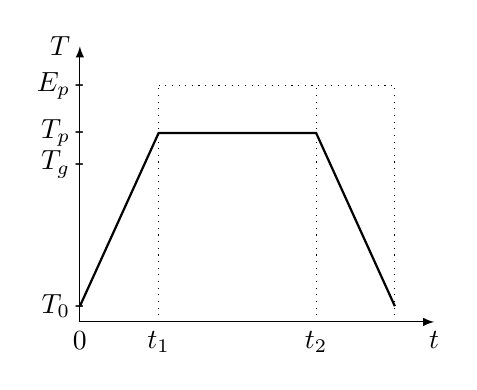
\begin{tikzpicture}

% horizontal axis
\draw[->] (0,0) -- (4.5,0) node[anchor=north] {$t$};
% labels
\draw	(0,0) node[anchor=north] {0}
		(1.0,0) node[anchor=north] {$t_1$}
		(3.0,0) node[anchor=north] {$t_2$};
% ranges
%\draw	(1,3.5) node{{\scriptsize Constant flux}}
%		(4,3.5) node{{\scriptsize Field weakening}};

% vertical axis
\draw[->] (0,0) -- (0,3.5) node[anchor=east] {$T$};
% labels
\draw	(0,0.2) node[anchor=east] {$T_0$}
		(0,0) node[anchor=south] {-}
		(0,2.0) node[anchor=east] {$T_g$}
		(0,1.8) node[anchor=south] {-}
		(0,2.4) node[anchor=east] {$T_p$}
		(0,2.2) node[anchor=south] {-}
		(0,3.0) node[anchor=east] {$E_p$}
		(0,2.8) node[anchor=south] {-};
% nominal speed
\draw[dotted] (1.0,0) -- (1.0,3.0);
\draw[dotted] (3.0,0) -- (3.0,3.0);
\draw[dotted] (4.0,0) -- (4.0,3.0);
\draw[dotted] (1.0,3.0) -- (4.0,3.0);
% Us
\draw[thick] (0,0.2) -- (1.0,2.4) -- (3,2.4) -- (4.0,0.2);
%\draw (1,1.5) node {$U_s$}; %label
%Y tick marks
%\foreach \x in {0,...,6}
%     		\draw (\x,1pt) -- (\x,-3pt)
%			node[anchor=north] {\x};
%    	\foreach \y in {0,...,4}
%     		\draw (1pt,\y) -- (-3pt,\y) 
%     			node[anchor=east] {\y}; 
% Psis
%\draw[thick,dashed] (0,3) -- (2,3) parabola[bend at end] (6,1);
%\draw (2.5,3) node {$\varPsi_s$}; %label

\end{tikzpicture}

\end{document}